% Pulse sequence (NMR / qubit timing) — pure TikZ.
\documentclass[border=4pt]{standalone}
\usepackage{tikz}
\usetikzlibrary{positioning}
\usepackage{amsmath}

% Luxas palette (figures v5) — generated from skills/figure/scripts/colorkey.py; keep in sync with it.
% Schematics: levels, state labels and text are BLACK. Colour goes on drive arrows by wavelength (beam*),
% and on an object only when it names an identity the report's data figures also use (lx<Family>, the
% family recorded for it in report/figures/colorkey.json). Tints: D dark (text), plain mid (lines),
% L light (fills), P pale (areas).
\definecolor{lxBlue}{HTML}{3B7CAE}\definecolor{lxBlueD}{HTML}{174F75}\definecolor{lxBlueL}{HTML}{A3C1E2}\definecolor{lxBlueP}{HTML}{E4ECF6}
\definecolor{lxRed}{HTML}{CA5852}\definecolor{lxRedD}{HTML}{892F2D}\definecolor{lxRedL}{HTML}{ECACA4}\definecolor{lxRedP}{HTML}{FCE6E3}
\definecolor{lxOrange}{HTML}{D17B3A}\definecolor{lxOrangeD}{HTML}{804619}\definecolor{lxOrangeL}{HTML}{F5C19F}\definecolor{lxOrangeP}{HTML}{FFEADD}
\definecolor{lxGreen}{HTML}{497E50}\definecolor{lxGreenD}{HTML}{2B5731}\definecolor{lxGreenL}{HTML}{A7CAA9}\definecolor{lxGreenP}{HTML}{E5F1E6}
\definecolor{lxPlum}{HTML}{8A6194}\definecolor{lxPlumD}{HTML}{62396D}\definecolor{lxPlumL}{HTML}{CAB1CF}\definecolor{lxPlumP}{HTML}{F1E8F2}
\definecolor{lxSand}{HTML}{AD8B55}\definecolor{lxSandD}{HTML}{6A5124}\definecolor{lxSandL}{HTML}{EACDA5}\definecolor{lxSandP}{HTML}{FBEFE0}
% drive colours by wavelength: beamUV <380 nm, beamViolet 380-440, beamBlue 440-495, beamGreen 495-570, beamAmber 570-605, beamOrange 605-660, beamRed 660-760, beamDeepRed 760-1000, beamIR >1 um
\definecolor{beamUV}{HTML}{7B3FA0}\definecolor{beamViolet}{HTML}{4E4BC0}\definecolor{beamBlue}{HTML}{2F6FC0}\definecolor{beamGreen}{HTML}{2E8B47}\definecolor{beamAmber}{HTML}{B07C00}\definecolor{beamOrange}{HTML}{E0561F}\definecolor{beamRed}{HTML}{C8302B}\definecolor{beamDeepRed}{HTML}{A3262A}\definecolor{beamIR}{HTML}{7A1F1F}
\definecolor{labelGray}{HTML}{6E6E6E}

\begin{document}
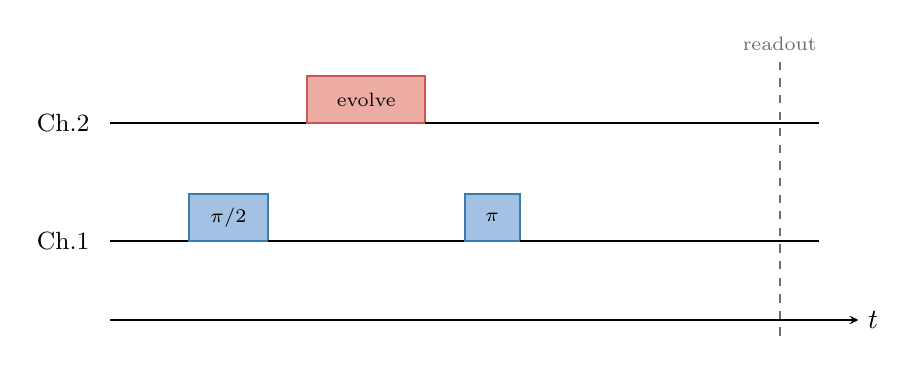
\begin{tikzpicture}[font=\sffamily, >=stealth]
  % Time axis
  \draw[->] (0,0) -- (9.5,0) node[right]{$t$};

  % Channel 1
  \node[left=4pt of {(0,1)}, font=\small] {Ch.1};
  \draw[thick] (0,1) -- (1,1);
  \draw[lxBlue, thick, fill=lxBlueL] (1,1) rectangle (2.0,1.6);
  \node[font=\scriptsize] at (1.5, 1.3) {$\pi/2$};
  \draw[thick] (2.0,1) -- (4.5,1);
  \draw[lxBlue, thick, fill=lxBlueL] (4.5,1) rectangle (5.2,1.6);
  \node[font=\scriptsize] at (4.85, 1.3) {$\pi$};
  \draw[thick] (5.2,1) -- (9,1);

  % Channel 2
  \node[left=4pt of {(0,2.5)}, font=\small] {Ch.2};
  \draw[thick] (0,2.5) -- (2.5,2.5);
  \draw[lxRed, thick, fill=lxRedL] (2.5,2.5) rectangle (4.0,3.1);
  \node[font=\scriptsize] at (3.25, 2.8) {evolve};
  \draw[thick] (4.0,2.5) -- (9,2.5);

  % Readout marker
  \draw[labelGray, thick, dashed] (8.5, -0.2) -- (8.5, 3.3);
  \node[labelGray, font=\scriptsize, above] at (8.5, 3.3) {readout};
\end{tikzpicture}
\end{document}
